\documentclass[15pt]{article}
\author{Zhixin Wang, Yijing Gong, Haowen Hu, Alex Radicia}
\title{Crashes in the City of Madison}

\date{}

\usepackage{tikz}
\usepackage{graphicx}
\usepackage{float}
\usepackage{hyperref}
\usepackage{color,soul}
\usepackage{rotating}
\usetikzlibrary{mindmap,trees}

\begin{document}
\maketitle

~\\
~\\
~\\
~\\
~\\
~\\
~\\
~\\
\section{Introduction}
During the years of 2000-2018 in the city of Madison, 40001 crashes were documented and resulted in 201 deaths. This study aimed to identify the common features of these crashes to guide safety improvement efforts. This report consists mainly of three sections: when, how, and where to comprehensively analyze factors that may be related to crashes.           
~\\
\newline
The data in this study was generated after carefully reviewing the crash report filed for each crash as well as the general purpose crash data file produced by the Wisconsin Department of Transportation (WisDOT), Bureau of Traffic Operations (BTO), and distributed by the Wisconsin Traffic Operations and Safety (TOPS) Laboratory at the University of Wisconsin-Madison.    

\newpage
\section{The highlights of our report}
~\\
1. A significant drop in the number of nighttime alcohol-related crashes was observed from year 2007 to year 2008, possibly caused by the release of a new policy (ALDO).
~\\
~\\
2. Alcohol-related crashes peaked at 2am on weekends when more than 40\% of total crashes was alcohol-related.
~\\
~\\
3. On weekdays, high crash rates associated with working hours (~8am and ~4pm). 
~\\
~\\
4. About half of the drivers (49\%) involved in alcohol-related crashes was aged from 21 to 35. In addition, there was 11\% of drunk drivers were under 21 years old. 
~\\
~\\
5. In terms of gender, about 70\% of drunk drivers were male.
~\\
~\\
6. Annual number of crashes maintained around 5000 cases, despite of population increase from 208 thousand to 258 thousand from 2000 to 2018. 
~\\
~\\
7. Top five crash types were parked vehicle (27\%), tree (9\%), traffic sign (5\%), pedestrian (5\%) and bike (5\%).
~\\
~\\
8. 60\% of the injuries happened on the 6\% of the streets, such as E Washington Ave and S Gammon Rd. 

\newpage
\section{When do crashes happen in Madison?}
\subsection{Week and Hour}
\label{sec:WH}
Figure 1 shows the rate at which accidents occur at different times of day, during the weekdays and weekend. (The curves from Monday to Friday are very similar @\ref{sec:WH1}.). The two peaks of the working day curve are 7am-8am and 4pm-6pm, which may be caused by the increase in traffic volume from commuting, in turn leading to an increase in the number of crashes in the City of Madison. In addition, it can be clearly seen from the figure that the number of crashes during off-hours (4pm-6pm) is higher than that of work hours. Since people start working at different times, usually ranging from 7am to 10am or even later, so the scattered working hours slow down the traffic on the road. But no matter what type of work, people will get off work from four to six, so the more amount of traffic during off hours leads to a higher number of accidents. 
\begin{figure}[H]
\centering
\includegraphics[height=85mm]{HourNM.eps}
\caption{\# of Weekly Crash Distributed by Hour in Madison}
\label{1}
\end{figure}
 And people may have just left the bar from midnight till 4 in the morning on the weekend, but most people stay home during that time on work-days. This should be the main reason why the weekend curve is higher than the work-day curve before 4 am. For the Alcohol-Related crashes, it can be concluded that the peak hours of drunk driving are between 0:00 and 3:00 AM, regardless of which day of the week. And we know that buses in Madison don't operate after midnight.

In order to solve this problem, we can refer to the weekend late-night bus service provided by some schools in New York State\footnote{Nazareth College, Rochester Institute of Technology, the State University College at Geneseo and the University of Rochester are among local colleges that have various late-night bus services - usually on weekend nights - to off-campus sites.}, or the popular chauffeur service in China\footnote{The company introduced Didi Chauffeur (or Didi Daijia in Chinese), a service that lets users summon temporary personal drivers. Car owners who find themselves physically unable to drive can tap one of Didi Kuaidi's apps, and a driver will head to the person's location and hop in their car. The most obvious use for the service is to provide designated drivers after a night out drinking. Designated drivers may opt to take public transportation to get back home, or bring a folding bike along. The company might provide shuttle buses for chauffeurs when demand is high. Or they could hitch a ride back using one of Didi’s other Uberesque services—like Didi Dache, which provides taxi rides.}.

\subsection{Month}
We took the top five types of crashes in Madison and looked at their monthly distribution. As can be seen from the figure, the most obvious pattern of crashes is bicycle accidents. With the increase of temperature, the number of accidents keeps increasing, while in the cold months, there is a significant decline. The number of crashes in the trough month is only 12.7\% of the peak month. The biggest type was the number of crashes involving parked vehicles, the spike in winter may be explained by slippery roads, while fluctuations in other months may be related to the number of parked vehicles or just the number of total crashes.
\begin{figure}[H]
\centering
\includegraphics[height=75mm]{MonthM.eps}
\caption{\# of Crash Distributed by Month}
\end{figure}

\newpage
\subsection{Year}
From the Figure 3, we can see that the number of drunk driving in Madison City suddenly dropped a lot in 2007(a new policy(ALDO)\footnote{ALDO forbids new tavern licenses inside the downtown area — bounded by Blair Street on the east, Park and Regent streets on the west, and the lakes on the north and south. People can still get liquor licenses there for new restaurants, but they are required to generate at least 50\% of their revenue from food sales.} to restrict the operation of Madison City bars was introduced), which leads to that total number of drunk driving in 2013 was only 50\% in 2007. This policy expired in 2011 and lowered the bar restrictions on the basis of the original policy\footnote{Under the compromise plan, up to seven new nightspots could open Downtown provided they draw no more than 65 percent of revenue from alcohol sales and focus primarily on entertaining patrons. Movies, music, theater, sports, bowling and arcade games all qualify.}for two year's extension, which is why the number of drunk drivers has increased.
\begin{figure}[H]
\centering
\includegraphics[height=80mm]{AYearcrashM.eps}
\caption{\# of Alcohol-Related Crash Distributed by Year}
\end{figure}
After 2013, the policy in 2011 has been expired. As an alternative to it, the city is looking at creating new zoning regulations\footnote{The new alcohol license ordinance creates a special zoning area for the 500 and 600 blocks of State Street, the north side of the 600 block of University Avenue, the 400 blocks of North Frances and West Gilman streets and west side of the 10 block of North Broom Street where there are many licenses and alcohol-related problems. No new taverns or new retail alcohol sales will be allowed in that area, but brew pubs, nightclubs and restaurant-nightclubs can be permitted as conditional uses.} for places that sell alcohol. The officials concede that ALDO (The main aim is to reduce drunk crime) in 2007 has failed because the number of drunk crime did not drop significantly, but there is no doubt that the policy does make a significant impact on drunk driving. In addition, the number of daytime crashes has barely changed, which is also a good indication of reducing the amount of drunk driving.

\section{How do crashes happen in Madison?}
\subsection{Age}
From Figure 4, we can see the age ratio of crashes in different hours. The rate of crashes among young people rises gradually after noon, and peaks in the early hours of the morning. Based on the previous analysis of drunk driving time, we've already known that the peak hours of drunk driving are between 0:00 and 3:00 AM. So we infer that drunk driving is mainly caused by young people in the 20s.
\begin{figure}[H]
\centering
\includegraphics[height=80mm]{AgeM.eps}
\caption{Age Distribution of Drivers in crashes}
\label{11}
\end{figure}

\newpage
\subsection{Gender}
Figure 5 shows the gender composition of drivers involved in crashes in the City of Madison from 2000 to 2018. We can see that no matter the total number of crashes or the number of drunk driving, male are higher than female. And although the total number fluctuates between years, the trend of men's lines and women's lines is very similar. 
\begin{figure}[H]
\centering
\includegraphics[height=80mm]{Gender.eps}
\caption{Gender Distribution of Drivers in Crashes}
\label{13}
\end{figure}

\newpage
\subsection{Types of crash}
Figure 6 shows the top five types of fatal crashes and their total number of crashes. Although crashes related to train has the highest fatal rate, but the total number of this type is extremely low. So we can say that the most dangerous type of crashes is which hits pedestrians. 
\begin{figure}[H]
\centering
\includegraphics[height=100mm]{TYPEF.eps}
\caption{\% Fatality Distributed by Type in Madison}
\label{16}
\end{figure}

\subsection{Severity}
\subsubsection{Speed and Severity}
Table 1 shows the percent of crashes in different speed limits at three different severity levels in the City of Madison. 

\begin{table}[htbp]
  \centering
  \caption{the correlation between severity and speed limits}
    \begin{tabular}{lrrrr}
    \hline
          & \multicolumn{1}{l}{0-25} & \multicolumn{1}{l}{30-40} & \multicolumn{1}{l}{45-55} & \multicolumn{1}{l}{60+} \\
    \hline
    Fatal & 0.24\% & 0.75\% & 1.42\% & 3.32\% \\
    In-capacitating & 13.52\% & 11.50\% & 15.69\% & 16.24\% \\
    Non-Incapacitating & 86.24\% & 87.75\% & 82.89\% & 80.44\% \\
    \hline
    \end{tabular}%
  \label{tab:addlabel}%
\end{table}%

We can say that for fatal crashes, the higher the speed limit, the greater the number. For minor injuries that are non-incapacitating, the lower the speed limit, the greater the number. For incapacitating accidents, there is no significant difference in the amount of occurrence between different speed limits.

\subsubsection{Age and Severity}
From Figure 7, the percentage of minor injuries and disabilities between different age groups fluctuates very little in the City of Madison. So we infer that there's no correlation between age and crashes that don't kill people. And we can see that the percentage of incapacitating accidents in the drunk driving is higher than that of all crahes and the percentage of non-incapacitating accidents is lower than that of all crahes, so we conclude that drunk driving accidents will cause more serious harm to the driver.
\begin{figure}[H]
\centering
\includegraphics[height=80mm]{AgeS.eps}
\caption{\% Severity Distributed by Age}
\label{19}
\end{figure}

From figure 8, we can see that among all accidents, crashes involving drivers aged 45-55 have the lowest fatality rates in the City of Madison. This might because drivers in this age group are more experienced than younger drivers and have quicker reflexes than older drivers. But in the case of drunk driving, crashes involving drivers aged 45-55 have the highest fatality rates. This may be because physical well-being declines with age and drunk driving are more likely to be fatal. However, older people over the age of 55 tend to be more cautious, so the fatality rate in drunk driving events is not high.
\begin{figure}[H]
\centering
\includegraphics[height=80mm]{AgeSF.eps}
\caption{\% Fatality Distributed by Age}
\label{21}
\end{figure}

~\\
~\\
~\\

\section{Where do crashes happen in Madison?}
\subsection{Year}
We observed a significant decline in the number of crashes associated with alcohol driving between the year of 2007 and 2008. Thus, we plotted out the crash maps from 2000 to 2007 vs. 2008 to 2013. Here on the maps, we can clearly tell that not only were there fewer crashes after 2007, but also on some of the streets where there used to be crashes, we can’t see any of those accidents any more.
\begin{figure}[H]
\raggedleft
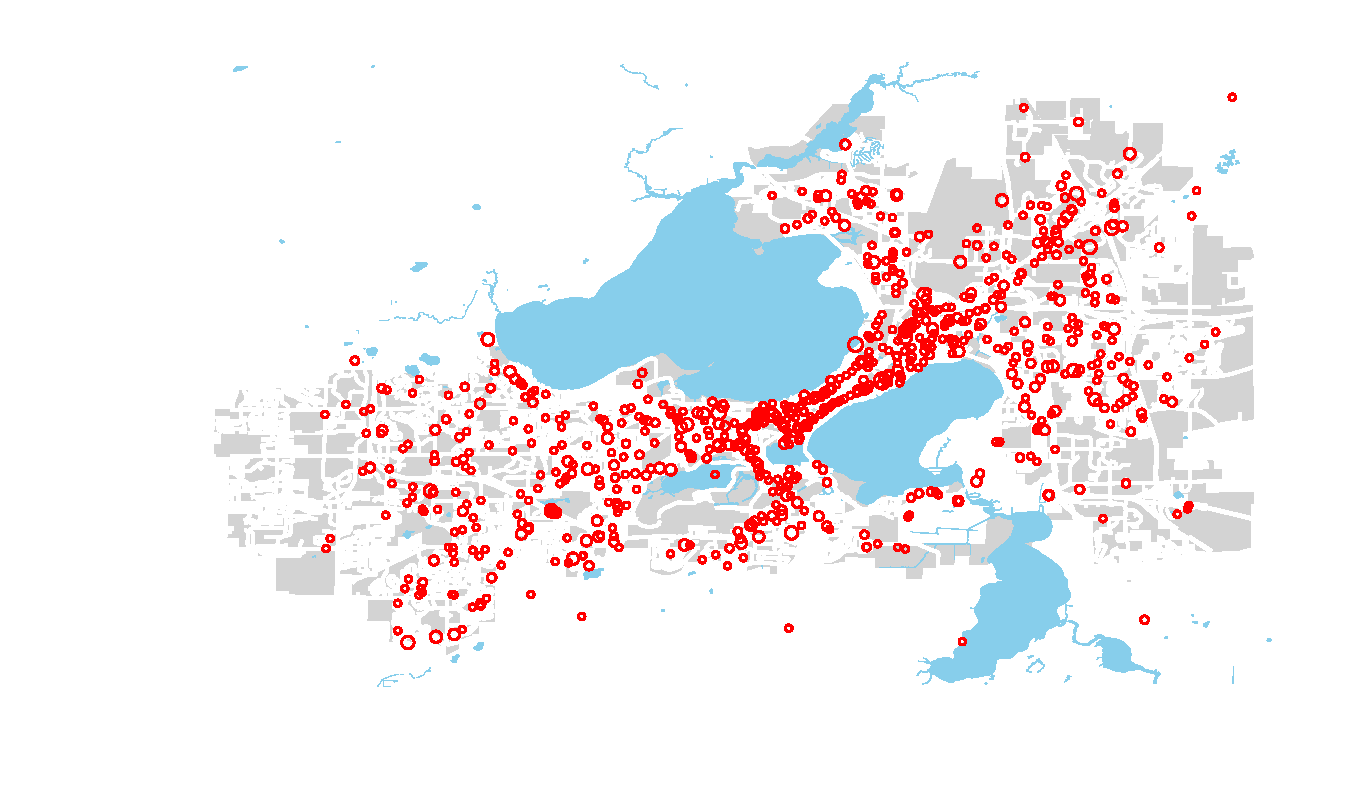
\includegraphics[height=80mm]{year1.eps}
\caption{Crashes in Madison before 2007}
\end{figure}

\begin{figure}[H]
\raggedleft
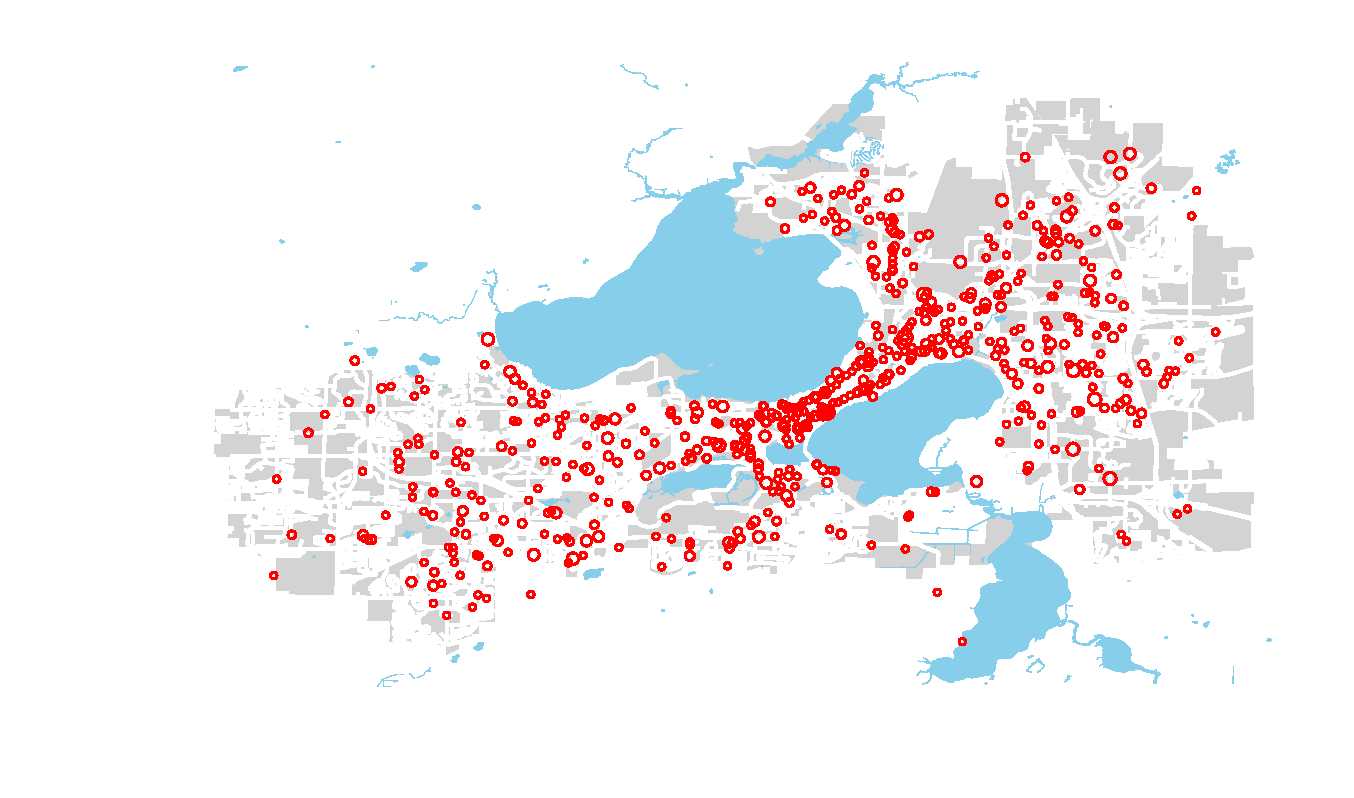
\includegraphics[height=80mm]{year2.eps}
\caption{Crashes in Madison after 2007}
\end{figure}


\subsection{Deer}
It is surprising that Madison has a high number of crash on deer (806 crashes over 19 years). Figure 11 shows the locations where crashes on deer have occurred in Madison over the past 19 years. As expected, The majority of crashes on deer have occurred on the periphery of Madison, and mainly in the northern part and around the Mendota Lake.
\begin{figure}[H]
\raggedleft
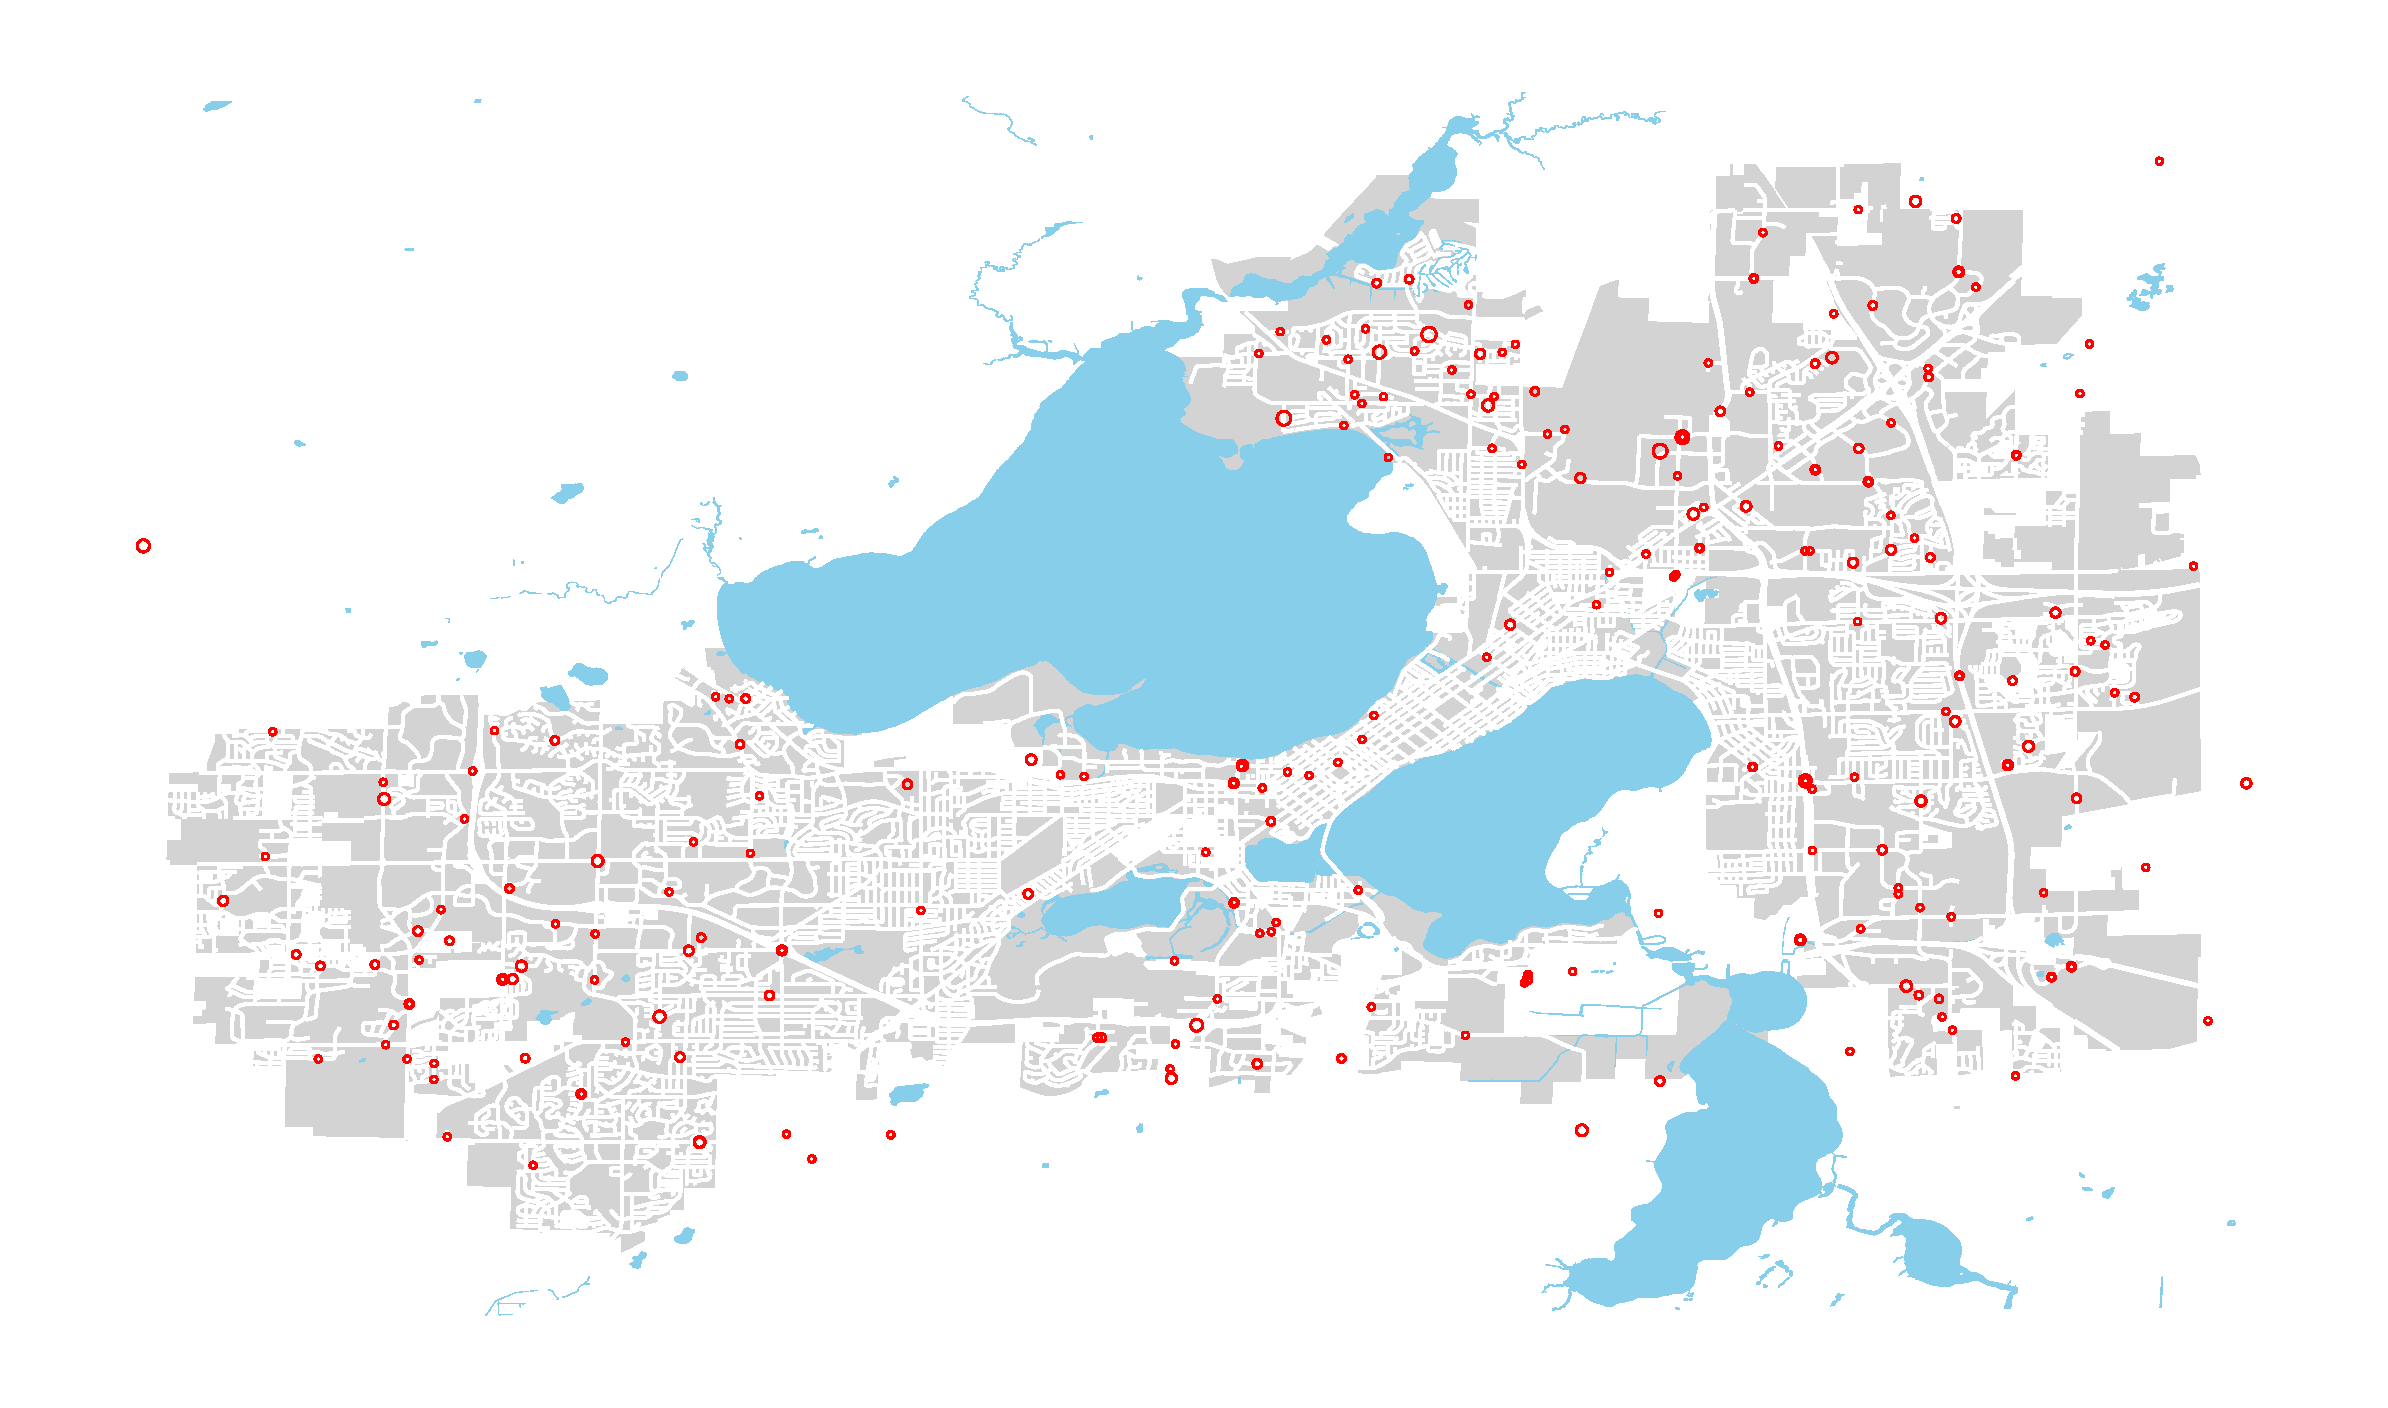
\includegraphics[height=80mm]{deer.eps}
\caption{Deer-Related crashes in Madison}
\end{figure}

~\\
~\\
\subsection{Bike and Pedestrian}
Figure 12 and Figure 13 show the locations where crashes have occurred in Madison over the past 19 years on bike (ranked fifth in types of crash) and pedestrian (ranked fourth), respectively. And our maps highly corrrespond with their crash maps. We found that bike crash map and pedestrian crash map shared a similar pattern where most of those crashes occurred in downtown Madison.
\begin{figure}[H]
\raggedleft
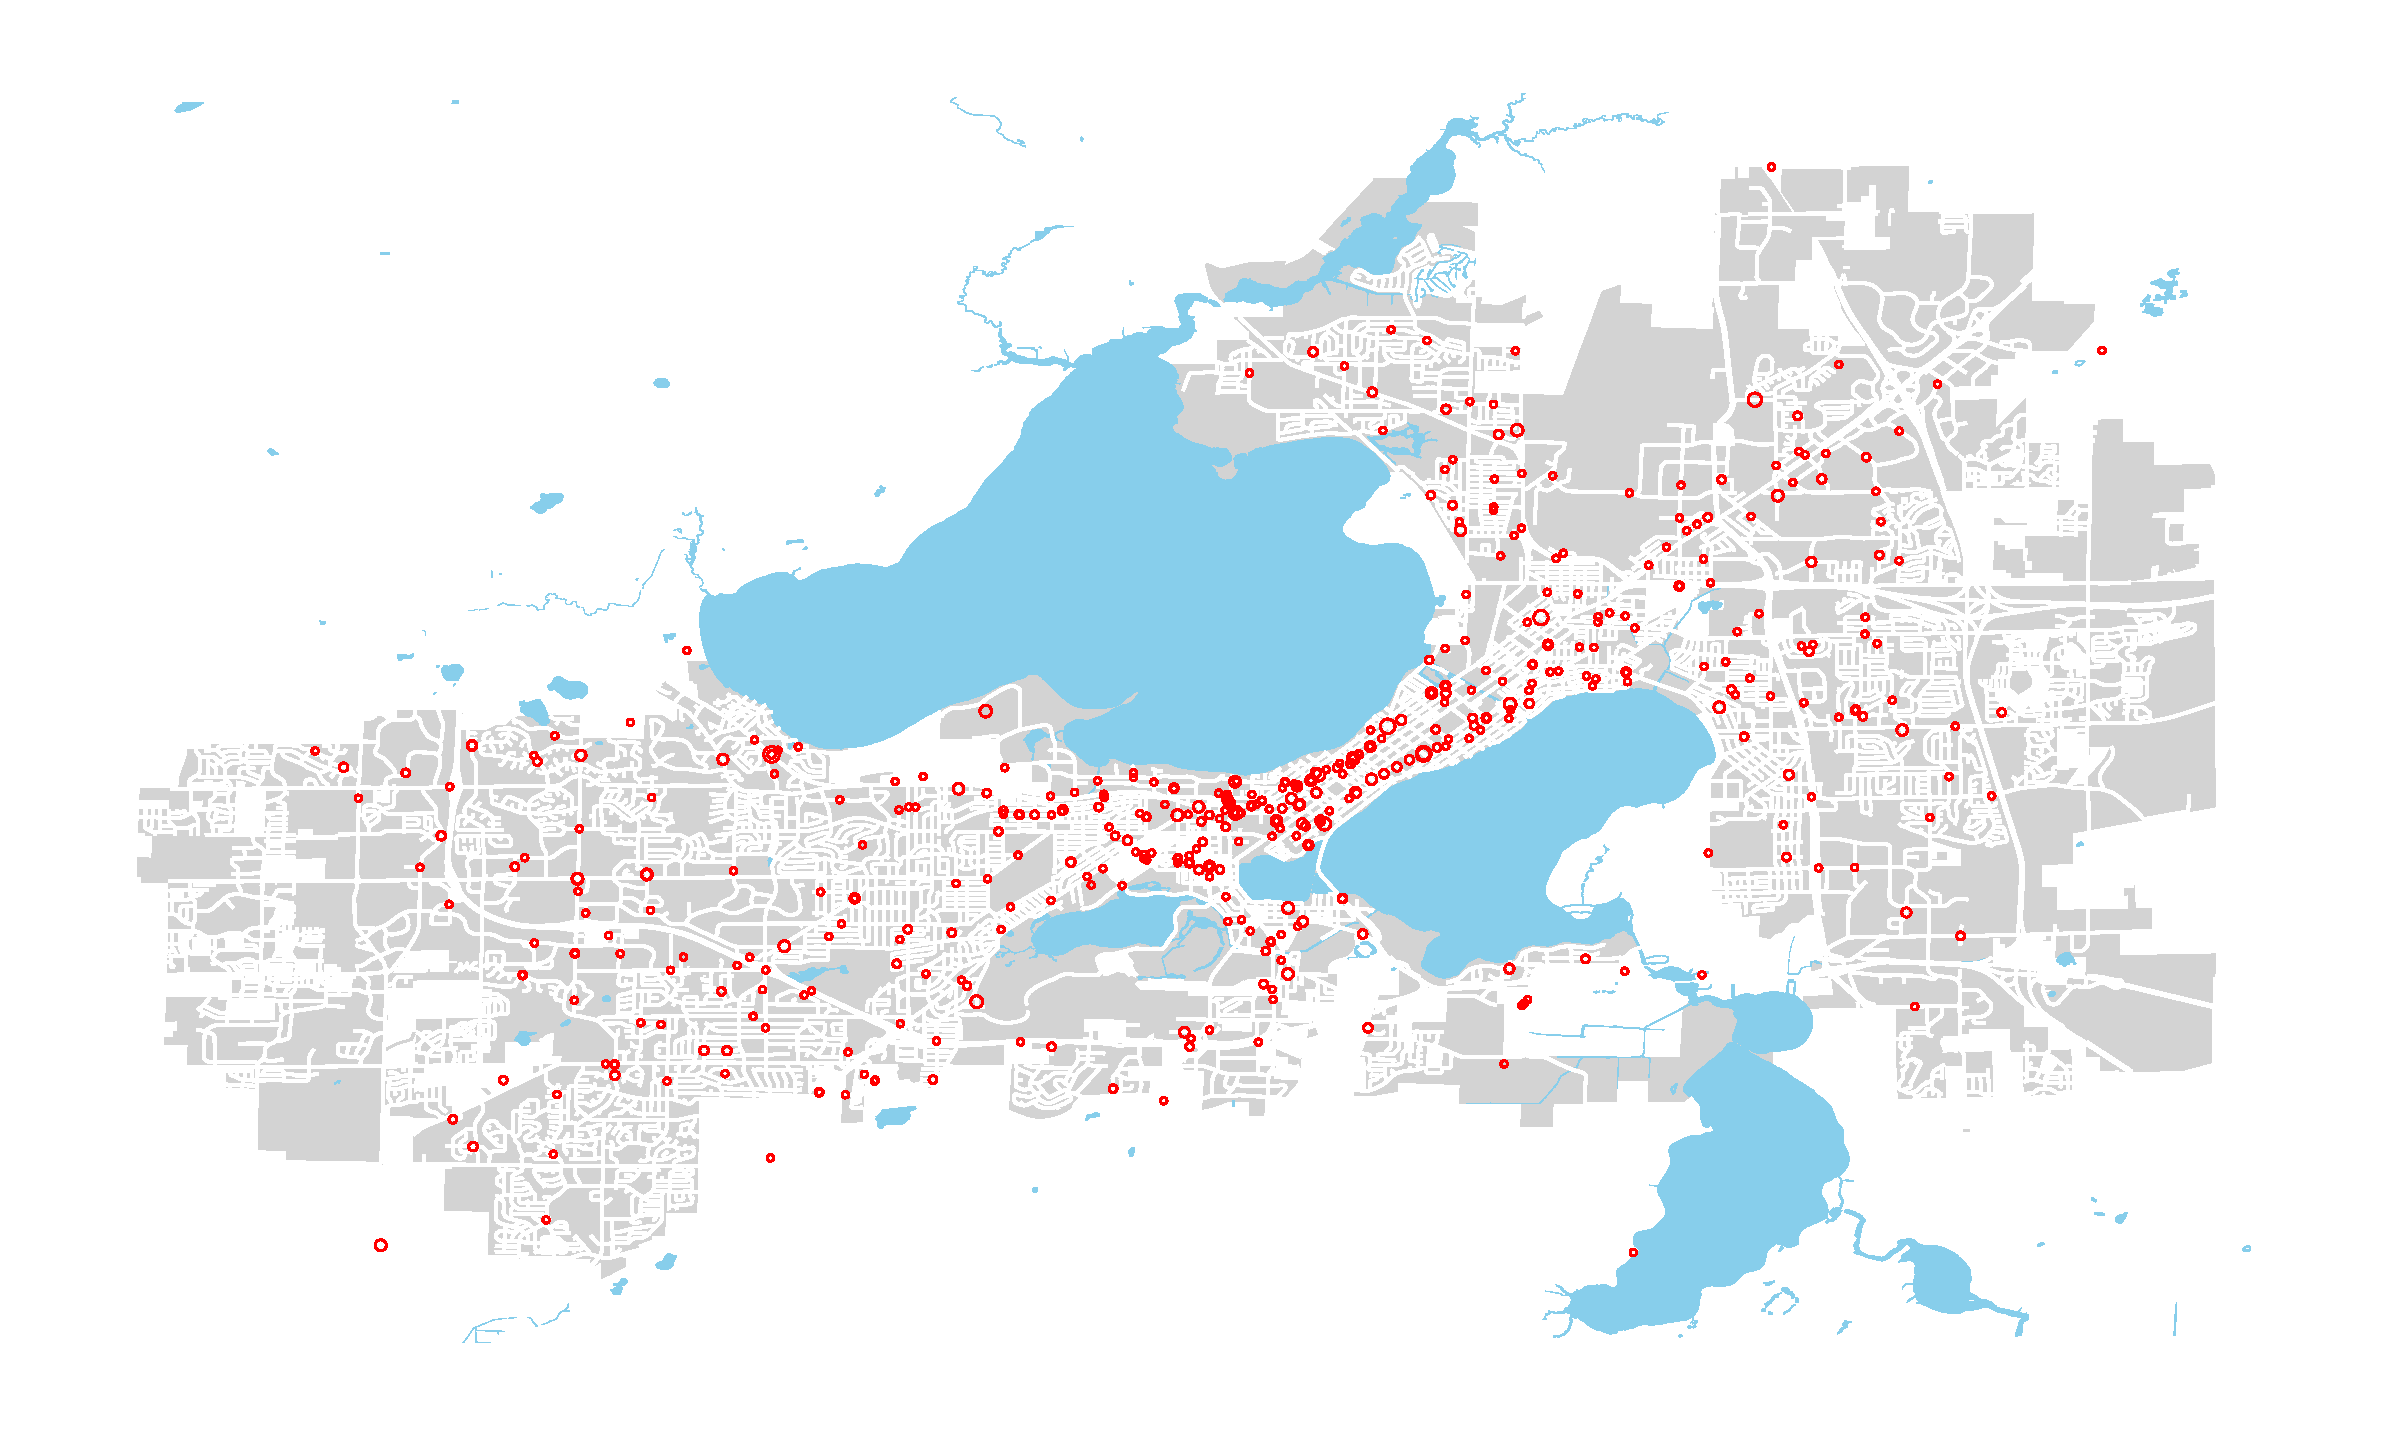
\includegraphics[height=68mm]{bike.eps}
\caption{Bike-Related crashes in Madison}
\end{figure}

\begin{figure}[H]
\raggedleft
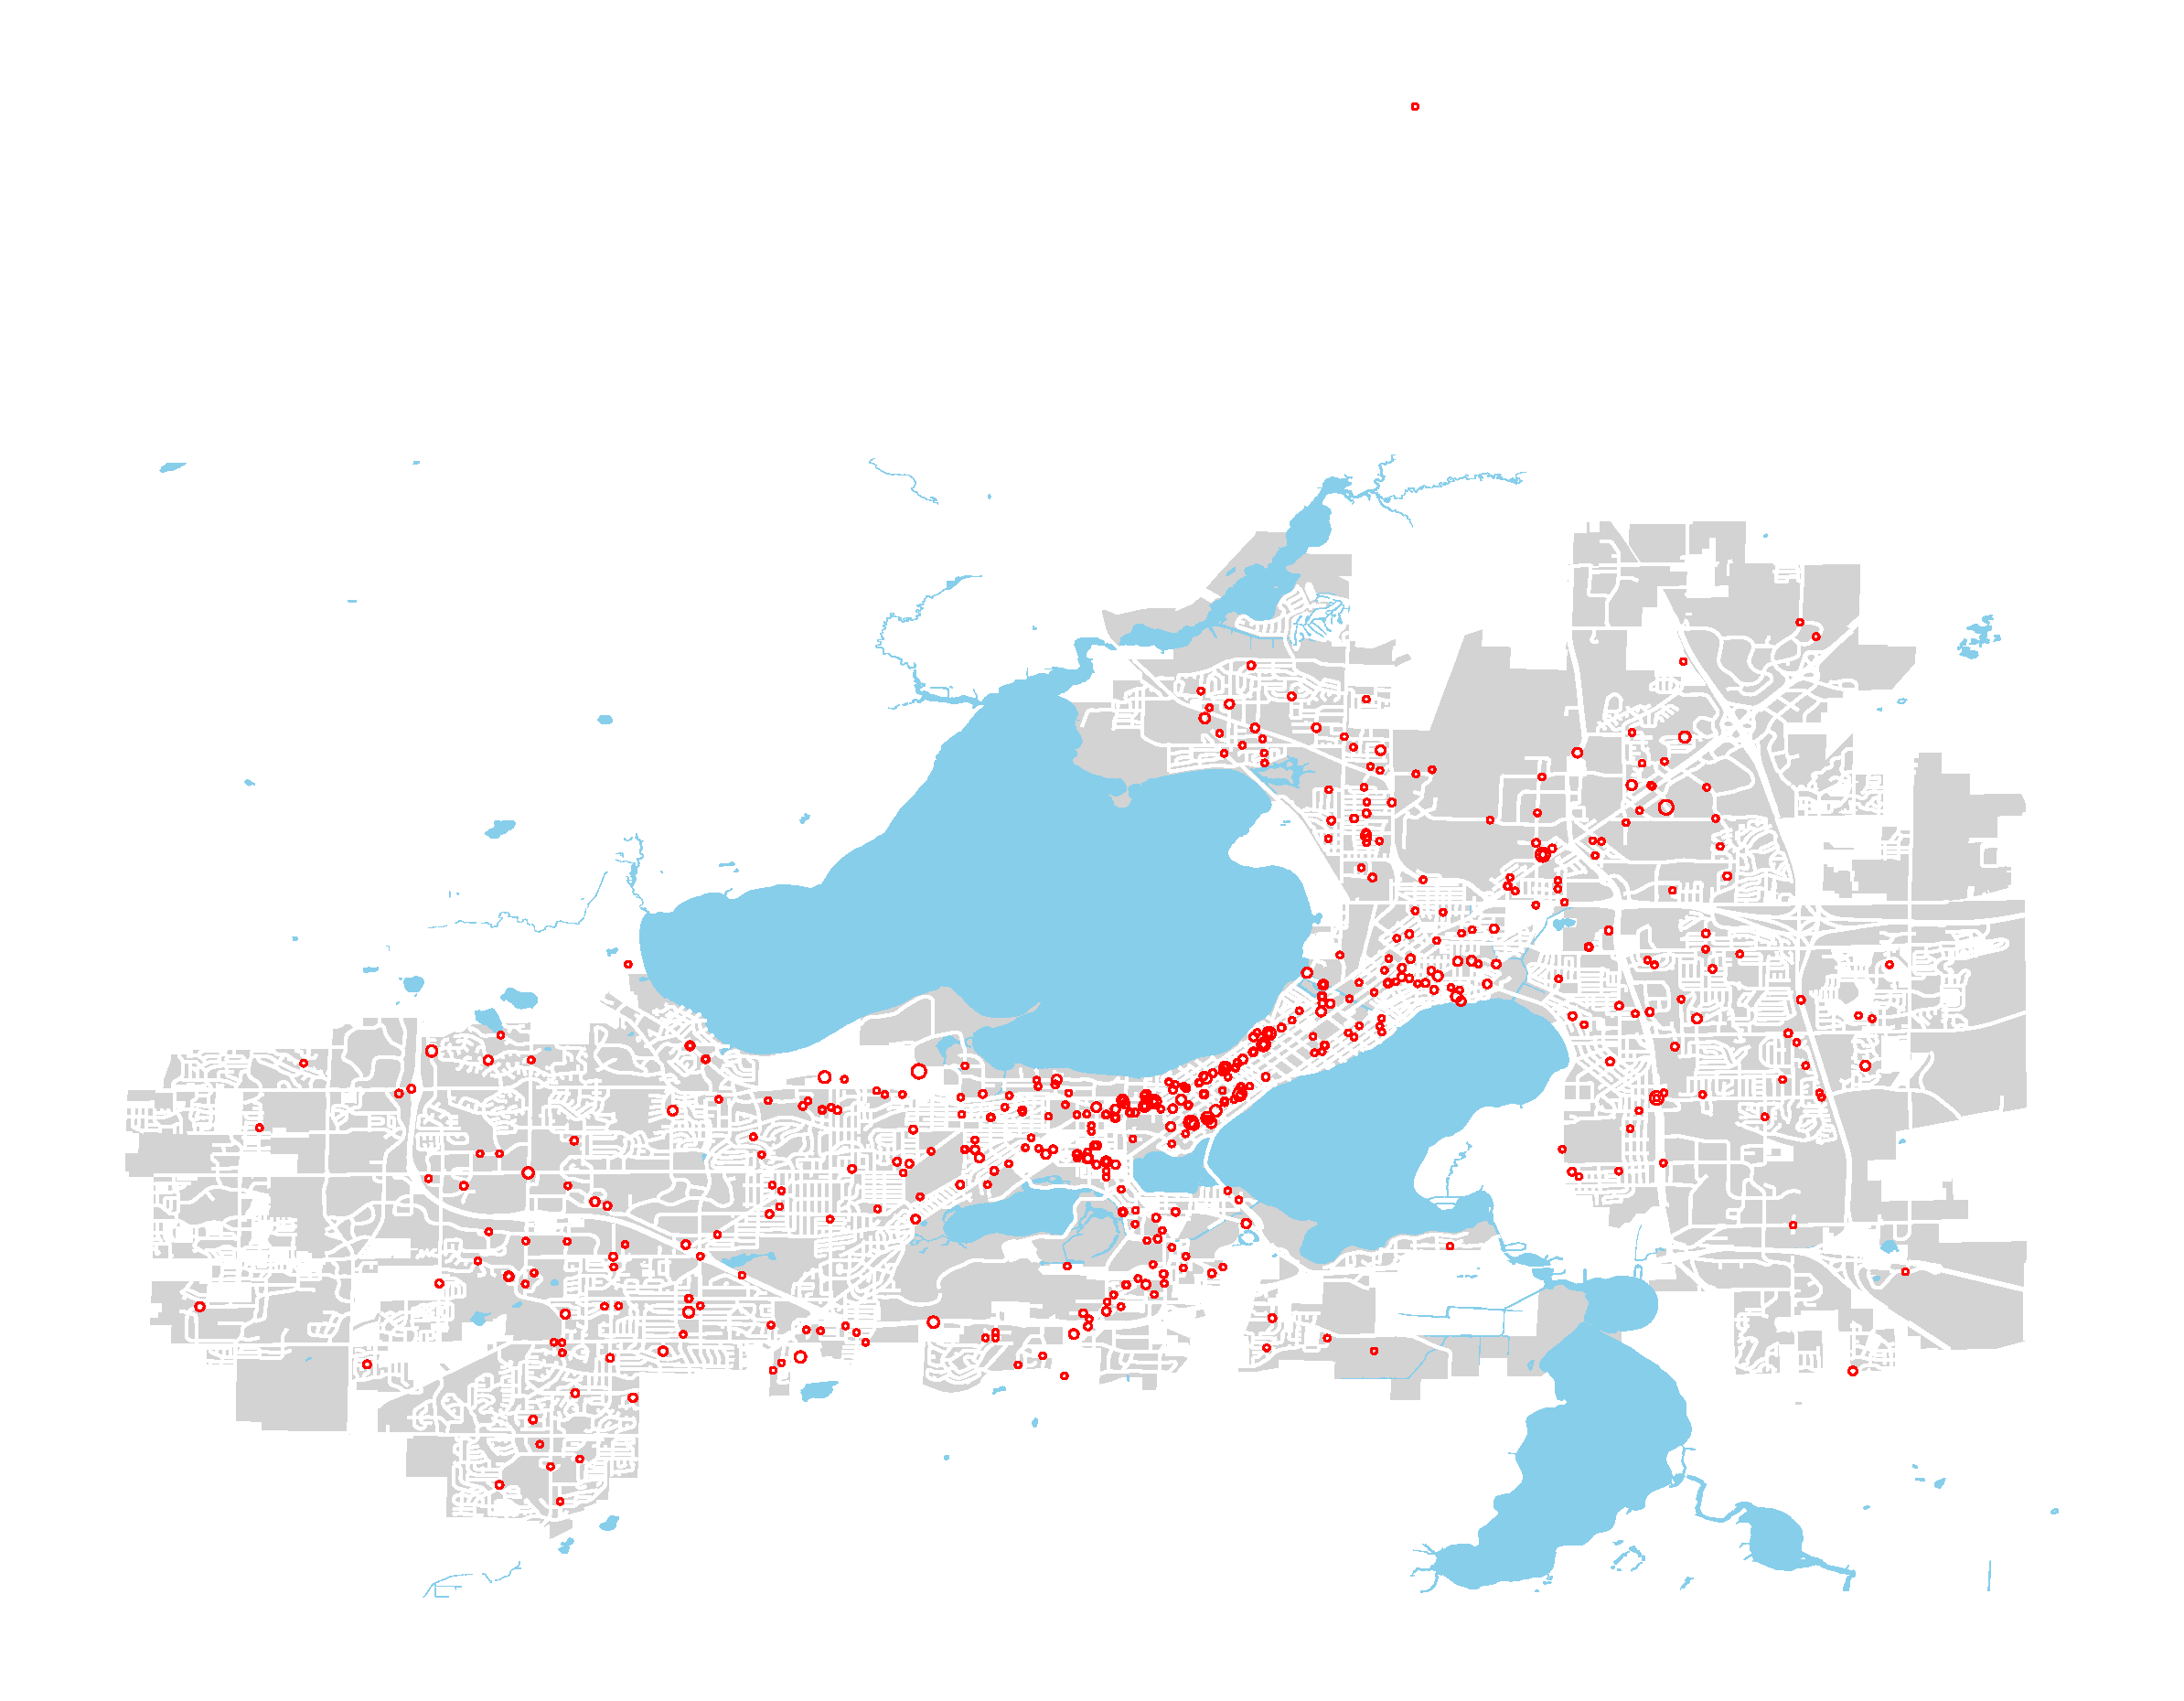
\includegraphics[height=85mm]{ped.eps}
\caption{Pedestrian-Related Crashes in Madison}
\end{figure}

\newpage
\subsection{More Information}
\begin{figure}[H]
\center
\includegraphics[width=130mm,height=72mm]{HourNMD.eps}
\caption{\# of Weekly Crash Distributed by Hour in Madison}
\label{sec:WH1}
\end{figure}

\begin{figure}[H]
\center
\includegraphics[width=130mm,height=72mm]{HourAMD.eps}
\caption{\% Weekly Alcohol-Related Crash Distributed by Hour in Madison}
\end{figure}

\end{document}